\documentclass[10pt]{article}

\usepackage{tikz}
\usepackage[version=4]{mhchem}

\begin{document}

% Overhang at the start and at the end.
\def\ppoverhang{0.3cm}
% Need one temporary variable which tells you how many cm the pulse sequence stretches to.
\newdimen\ppx
\ppx=0cm
\def\pppulsewidth{0.2cm}
\def\ppdelaywidth{1cm} % Need to figure out how to set this based on the size of #1.
\def\pppulseheight{0.8cm}
\def\ppfidwidth{1cm}

\def\ppdrawfullpulse#1{
    \draw[thick, fill=black] (\ppx,0) rectangle (\pppulsewidth + \ppx, \pppulseheight) ;
    \node[above] at (\pppulsewidth*0.5 + \ppx, \pppulseheight) {#1};
    \advance\ppx by \pppulsewidth
}

\def\ppdrawemptypulse#1{
    \draw[thick] (\ppx,0) rectangle (\pppulsewidth + \ppx, \pppulseheight) ;
    \node[above] at (\pppulsewidth*0.5 + \ppx, \pppulseheight) {#1};
    \advance\ppx by \pppulsewidth
}

\def\ppdrawdelay#1{
    \node at (\ppdelaywidth*0.5 + \ppx, \pppulseheight*0.5) {#1};
    \advance\ppx by \ppdelaywidth
}

\def\ppdrawacquisition{
    \draw[thick, xshift=\ppx] plot[smooth] coordinates { (0.0, 0.6) (0.041666666666666664, 0.3798293252415584) (0.08333333333333333, -0.07112559439940216) (0.125, -0.43951180429468606) (0.16666666666666666, -0.4910262010054742) (0.20833333333333331, -0.21731678797446832) (0.25, 0.1766216172050586) (0.29166666666666663, 0.4235613292679947) (0.3333333333333333, 0.3737703139019543) (0.375, 0.08353451850302532) (0.41666666666666663, -0.23812242366846623) (0.4583333333333333, -0.37834173220038547) (0.5, -0.2599344102804792) (0.5416666666666666, 0.018988825319158385) (0.5833333333333333, 0.2631929113755407) (0.625, 0.3157573904451798) (0.6666666666666666, 0.15763055376166304) (0.7083333333333333, -0.09093513388119927) (0.75, -0.2601598790395012) (0.7916666666666666, -0.2457234756806965) (0.8333333333333333, -0.07175129625843182) (0.875, 0.13523235653317198) (0.9166666666666666, 0.23723176180771896) (0.9583333333333333, 0.1759388257388005) (1.0, 0.004491994123336265) } ;
    \advance\ppx by \ppfidwidth
}

\def\ppdrawchannelline#1{
    \draw[thick] (-\ppoverhang, 0) node[left, text depth=0.4ex] {#1}
        -- (\ppx + \ppoverhang, 0) ;
}

2D J spectrum:

\begin{tikzpicture}
    % a 90deg pulse
    \ppdrawfullpulse{$\phi_1$}
    % a delay
    \ppdrawdelay{$\frac{t_1}{2}$}
    % a 180deg pulse
    \ppdrawemptypulse{$\phi_2$}
    % another delay
    \ppdrawdelay{$\frac{t_1}{2}$}
    % receiver
    \ppdrawacquisition
    % axis for a nucleus
    \ppdrawchannelline{\ce{^1H}}
\end{tikzpicture}

Carbon 1D spectrum:

\begin{tikzpicture}
    \ppdrawfullpulse{$\beta_x$}
    \ppdrawacquisition
    \ppdrawchannelline{\ce{^{13}C}}
\end{tikzpicture}

\end{document}
